\section{Rechnerarchitekturen}
\subsection{Von-Neumann-Architektur}

\begin{defi}{Von-Neumann-Architektur}
    Im Grundsatz besteht die Architektur aus drei Komponenten: \emph{CPU}, \emph{Speicher} und \emph{I/O Einheit}.

    Die einzelnen Komponenten sind über Datenleitungen, sogenannte \emph{Busse}, verbunden.
    \begin{center}
        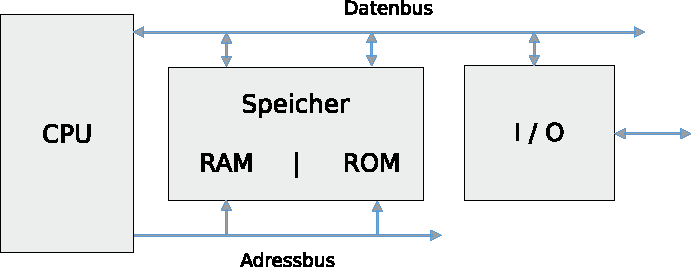
\includegraphics[]{images/von_neumann.pdf}
    \end{center}
\end{defi}

\begin{defi}{CPU}
    Die \emph{CPU} (\emph{Central Processing Unit}, Prozessor) ist sozusagen das Gehirn des Computers.
    Die CPU besteht im Wesentlichen aus drei Teilen, dem \emph{Leitwerk} und
    dem \emph{Rechenwerk} und den \emph{Registern}, welche direkt zur Abarbeitung von Befehlen
    benötigte Daten und berechnete Ergebnisse aufnehmen können.

    Das \emph{Leitwerk} steuert die Ausführung des Binärcodes, das \emph{Rechenwerk} führt anfallende Rechenoperationen aus.
\end{defi}

\begin{bonus}{Aufbau Rechenoperationen}
    \begin{itemize}
        \item \emph{Operationsteil}: codiert konkreten Befehl
        \item \emph{Operanden}: stellen z.B. Summanden einer Operation, oder Adresse einer Variablen dar
    \end{itemize}
\end{bonus}

\begin{bonus}{Abarbeitung von Befehlen}
    Jeder Befehl durchläuft bei der Abarbeitung in der CPU folgende Schritte:
    \begin{itemize}
        \item \emph{Instruction Fetch (IF)} : Befehl lesen
        \item \emph{Instruction Decode (ID)} : Befehl decodieren
        \item \emph{Fetch Operands (FO)} : Operanden laden
        \item \emph{Execute (EX)} : Befehl ausführen
        \item \emph{Writeback (WB)} : Ergebnis schreiben
    \end{itemize}

    \begin{center}
        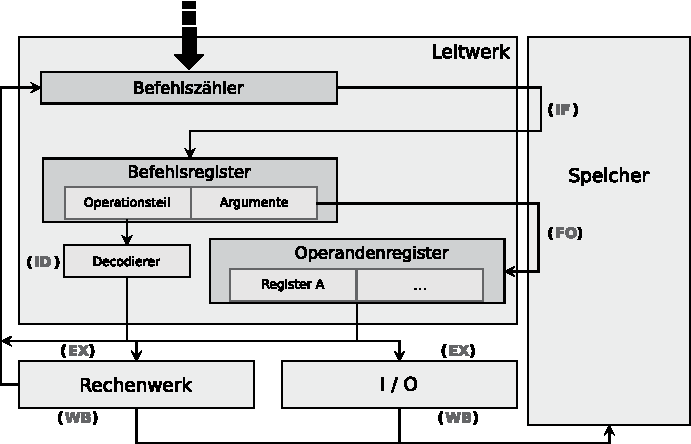
\includegraphics[]{images/befehlsabarbeitung.pdf}
    \end{center}
\end{bonus}

\begin{defi}{Prozessorarchitekturen}
    \textbf{CISC} (\emph{Complex Instruction Set Computer}):\\
    Eine CISC CPU zeichnet sich durch einen \emph{komplexen Befehlssatz} in Form von \emph{Microcode} und dem Vorhandensein nur \emph{weniger Register} aus.

    \textbf{RISC} (\emph{Reduced Instruction Set Computer}):\\
    eine RISC CPU nur über \emph{wenige, in Hardware realisierte Befehle} und \emph{viele Prozessorregister}.
\end{defi}

\begin{defi}{Pipelining}
    In einer \emph{RISC CPU}, die nur wenige und elementare Befehle verwendet, kann dafür
    gesorgt werden, dass alle Teilschritte, deren \emph{parallele Verarbeitung} das Pipelining
    ermöglicht, gleich lange dauern. Nur deswegen kann das Konzept des Pipelinings
    erfolgreich umgesetzt werden.

    Das ist bei einer \emph{CISC CPU} aufgrund der vielen
    und teils sehr komplexen Befehle \emph{nicht} möglich.
\end{defi}

\begin{example}{Pipelining}
    5-Stage-Pipeline:
    \begin{itemize}
        \item Instruction Fetch (\textbf{IF}): Befehl lesen
        \item Instruction Decode (\textbf{ID}) : Befehl decodieren
        \item Execute (\textbf{EX}) : Ausführen
        \item Memory Access (\textbf{MEM}) : Ausführen
        \item Writeback (\textbf{WB}) : Ergebnis schreiben
    \end{itemize}

    \begin{center}
        \begin{tabular}{| c || m{0.05\textwidth} | m{0.05\textwidth} | m{0.05\textwidth} | m{0.05\textwidth} | m{0.05\textwidth} | m{0.05\textwidth} |}
            \hline
            Instr. 1    & \texttt{IF}            & \texttt{ID}            & \texttt{EX}            & \texttt{MEM}           & \texttt{WB}            &                        \\
            \hline
            Instr. 2    &                        & \texttt{IF}            & \texttt{ID}            & \texttt{EX}            & \texttt{MEM}           & \texttt{WB}            \\
            \hline
            Instr. 3    &                        &                        & \texttt{IF}            & \texttt{ID}            & \texttt{EX}            & \texttt{MEM}           \\
            \hline
            Instr. 4    &                        &                        &                        & \texttt{IF}            & \texttt{ID}            & \texttt{EX}            \\
            \hline
            Instr. 5    &                        &                        &                        &                        & \texttt{IF}            & \texttt{ID}            \\
            \hline
            \hline
            Clock Cycle & \multicolumn{1}{c|}{1} & \multicolumn{1}{c|}{2} & \multicolumn{1}{c|}{3} & \multicolumn{1}{c|}{4} & \multicolumn{1}{c|}{5} & \multicolumn{1}{c|}{6} \\
            \hline
        \end{tabular}
    \end{center}
\end{example}

\begin{defi}{ROM}
    Der \emph{ROM} ist ein Festwertspeicher, der - prinzipiell - \emph{nur gelesen} werden kann und die Firmware des Computers gespeichert hat.

    Im ROM liegt das sogenannte \emph{BIOS} (\emph{basic input output system}) bzw. moderner \emph{UEFI}
    (\emph{unified extensible firmware interface}).
    Die im ROM abgelegten Informationen stellen die Firmware des
    Rechners dar. Diese Firmware sorgt dafür, dass der Computer nach dem Einschalten
    in die Lage versetzt wird, grundlegende Hardwarekomponenten zu verwalten.
\end{defi}

\begin{defi}{RAM}
    Der \emph{RAM},
    auch \emph{Hauptspeicher} genannt, ist ein Speicher mit \emph{wahlfreiem Zugriff}, der seinen
    Inhalt jedoch bei Verlust der Betriebsspannung \emph{verliert}. Im RAM werden Informationen
    abgelegt, die ein \emph{Programm zur Laufzeit} benötigt.

    Sollen Daten
    über das Ende des Programms hinaus gespeichert werden, müssen sie über die
    \emph{I/O-Einheit} auf einen anderen Speicher geschrieben werden.
\end{defi}

\begin{defi}{Cache}
    \emph{Cache} ist \emph{schneller} als RAM, kann aber nur \emph{weniger Speicherkapazität} zur Verfügung stellen.

    Das bedeutet, dass der Cache nur kleine Datenmengen, sogenannte \emph{Cacheblocks}, aus dem Hauptspeicher vorhalten kann.
    Diese haben eine definierte Größe und können dann schneller in die CPU geldaden werden, als das aus dem RAM möglich wäre.
\end{defi}

\begin{defi}{Lokalität}
    \textbf{Zeitliche Lokalität}:\\
    Es ist, bei entsprechender Programmierung, sehr wahrscheinlich, dass
    auf eine Speicherzelle nicht nur einmal, sondern in kurzer Zeit \emph{mehrmals zugegriffen}
    wird.

    \textbf{Örtliche Lokalität}:\\
    Es ist, bei entsprechender Programmierung, sehr wahrscheinlich, dass nach
    dem Zugriff auf eine bestimmte Speicherzelle auch ein \emph{Zugriff in deren unmittelbarer
        \glqq Nachbarschaft\grqq} stattfindet.
\end{defi}

\begin{bonus}{Aufbau eines Caches}
    \begin{center}
        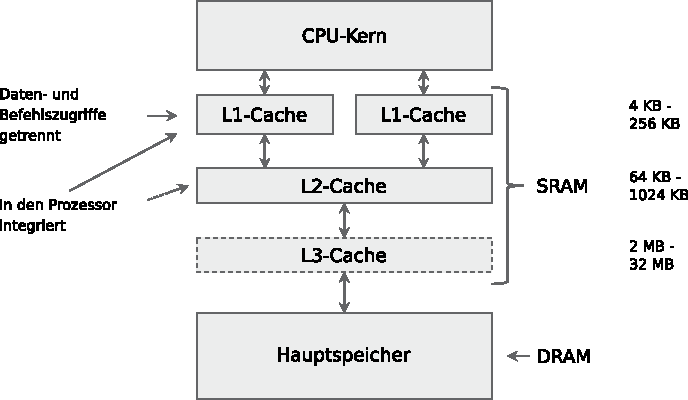
\includegraphics[]{images/cache_aufbau.pdf}
    \end{center}

    Aus der Abbildung ist ersichtlich, dass der Cache selbst ebenenweise organisiert ist.

    Im Regelfall sind mindestens die Ebenen L1 und L2 vorhanden, oftmals sogar noch
    eine dritte Ebene L3. Dabei ist in jedem Fall der L1-Cache in die CPU integriert,
    häufig auch noch der L2-Cache.

    Beginnend beim
    L3-Cache werden die Cachelevel mit größerer Nähe zur CPU jeweils kleiner und
    schneller. Dieser Aufbau soll die Frage nach der Auswahl der Daten, die im Cache
    vorgehalten werden, vereinfachen. Es ist also möglich einen relativ großen Datenbestand
    im L3-Cache vorzuhalten, der schneller ist als der Hauptspeicher. Von dort
    aus kann dann wiederum eine Teilmenge der Daten im noch schnelleren L2-Cache
    vorgehalten werden, usw.

    Liegen benötigte Daten nicht im L1-Cache, welcher Daten bzw. Befehle schlussendlich an die CPU liefert, ist aufgrund der Lokalität und
    des Aufbaus des Caches die Wahrscheinlichkeit hoch, dass die benötigten Daten
    nicht aus dem langsamen Hauptspeicher geladen werden müssen, sondern sich in
    einem der niedrigeren Cache-Level finden und damit immer noch vergleichsweise
    schnell zur Verfügung gestellt werden können.
\end{bonus}

\begin{bonus}{Interner Aufbau eines Cachelevels}
    \begin{center}
        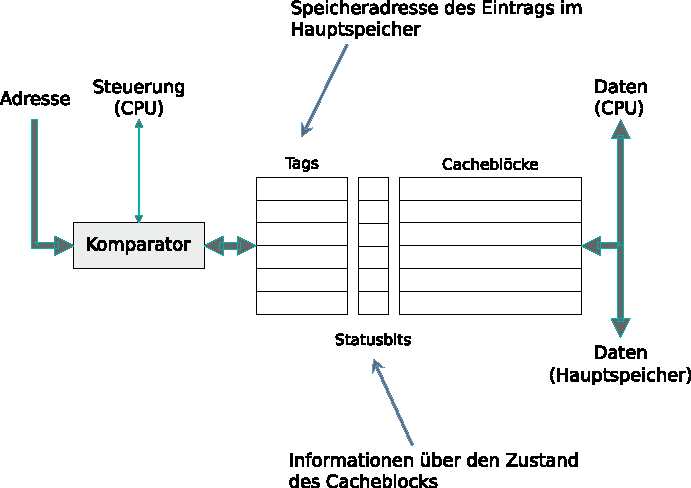
\includegraphics[]{images/cache_level.pdf}
    \end{center}

    Zu jedem Cacheblock wird die Startadresse des Blocks im RAM gespeichert, diese
    Information wird \emph{Tag} genannt.

    Wird von der CPU eine Anfrage an den Speicher
    gestellt, wird zunächst anhand des Tags unter Zuhilfenahme des Komparators geprüft, ob der angefragte Datensatz im Cache liegt. Dabei wird auch geprüft, ob eine
    angefragte Speicheradresse innerhalb eines Cacheblocks liegt. Das ist möglich, da
    der Tag sowie die Größe des Cacheblocks bekannt sind.

    Ist dies nicht der Fall, wird
    die Anfrage an ein niedrigeres Cachelevel bzw. den RAM weitergereicht.

    Außerdem
    werden zu jedem Cacheblock Statusbits gespeichert, die beispielsweise angeben ob
    sich der Cacheblock verändert hat (\emph{dirty bit}), seit er in den Cache geladen wurden,
    oder ob ein Platz im Cache mit einem gültigen Cacheblock belegt ist (\emph{invalid bit}).
\end{bonus}

\begin{defi}{Organisation der Tags}
    Die \emph{Blöcke} (Cache-Lines) eines Caches können in so genannte \emph{Sätze} zusammengefasst werden.
    Für eine bestimmte Adresse ist dann immer nur einer der Sätze zuständig.
    Innerhalb eines \emph{Satzes} bedienen alle Blöcke also nur einen \emph{Teil} aller vorhandenen Adressen.

    Im Folgenden stehe die Variable $m$ für die \emph{Gesamtanzahl der Cacheblöcke} und $n$ für die \emph{Anzahl der Blöcke pro Satz}, die so genannte \emph{Assoziativität}.
    Dann besteht der Cache also aus $\frac {m}{n}$ Sätzen.

    \textbf{Direkt abgebildet} (\emph{DM}, \emph{direct mapped}, $n=1$):\\
    Es gibt pro Cacheblock nur eine einzige Möglichkeit, wo dieser
    platziert werden kann.

    Daher kann es allerdings vorkommen, dass ein Cacheblock
    nicht platziert werden kann, obwohl noch Platz im Cache wäre.

    \textbf{Vollassoziativ} (\emph{FA}, \emph{fully associative}, $n=m$):\\
    Ein Cacheblock kann beliebige auf freie Plätze im Cache zugeordnet
    werden.

    Bei einer Speicheranfrage müssen allerdings alle gespeicherten
    Tags durchsucht werden.

    \textbf{Satzassoziativ} (\emph{SA}, \emph{set associative}, $2\leq n \leq \frac{m}{2}$):\\
    Der verfügbare Platz wird in Gruppen unterteilt. Wie bei einem
    DA Cache gibt es nur eine Gruppe, in der ein Cacheblock platziert werden kann;
    wie bei einem VA Cache kann der Cacheblock innerhalb dieser Gruppe frei platziert
    werden.
\end{defi}

\begin{defi}{Cache-Lesezugriffe}
    Findet ein Lesezugriff auf Speicherzelle $A$ statt, wird geprüft, ob Speicherzelle $A$ bereits im Cache liegt.
    \begin{itemize}
        \item \textbf{$A$ liegt im Cache} (\emph{cache hit}):\\
              Datensatz kann direkt aus dem Cache gelesen werden.
        \item \textbf{$A$ liegt nicht im Cache} (\emph{cache miss}):\\
              Datensatz muss aus dem Hauptspeicher in den Cache geladen werden, danach wird der Datensatz gelesen.
    \end{itemize}
\end{defi}

\begin{defi}{Schreibmodi eines Cache}
    \begin{itemize}
        \item \textbf{write-through} (\emph{WT}):\\
              Datensatz wird im Cache und direkt im Hauptspeicher aktualisiert.

              \emph{Vorteile}: keine Probleme mit Datenkonsistenz im Hauptspeicher\\
              \emph{Nachteile}: hoher Aufwand für Schreiboperationen
        \item \textbf{write-back} (\emph{WB}):\\
              Datensatz wird im Cache aktualisiert und erst dann in den Hauptspeicher geschrieben, wenn der entsprechende Cacheblock aus dem Cache verdrängt wird.

              \emph{Vorteile}: niedrige Belastund der Systembusse, keine Wartezyklen\\
              \emph{Nachteile}: fehlende Datenkonsistenz
    \end{itemize}
\end{defi}

\begin{defi}{Cache-Schreibzugriffe}
    Findet ein Schreibzugriff auf Speicherzelle $A$ statt, wird geprüft, ob Speicherzelle $A$ bereits im Cache liegt.
    \begin{itemize}
        \item \textbf{$A$ liegt im Cache} (\emph{cache hit}):\\
              Datensatz wird im Cache (und im Hauptspeicher) aktualisiert.
        \item \textbf{$A$ liegt nicht im Cache} (\emph{cache miss}):\\
              Datensatz wird im Hauptspeicher geschrieben, Inhalt des Caches wird nicht verändert.
    \end{itemize}
\end{defi}

\begin{defi}{Cache Misses}
    \begin{itemize}
        \item \textbf{Capacity Miss}:
              \subitem - tritt auf, wenn Datensatz bereits im Cache war, aber \emph{bereits verdrängt} wurde
              \subitem (aufgrund mangelnder Kapazität)
              \subitem - hauptsächlich bei VA Caches
        \item \textbf{Compulsory Miss}:
              \subitem - tritt auf, wenn ein Datensatz das \emph{erste Mal} verwendet wird
              \subitem - unabhängig vom Typ des Caches
        \item \textbf{Conflict Miss}:
              \subitem - tritt auf, wenn Datensatz bereits im Cache war, aber \emph{bereits verdrängt} wurde
              \subitem (weil ein anderer Cacheblock an entsprechende Stelle gelagert werden sollte)
              \subitem - vor allem bei DA Caches
    \end{itemize}
\end{defi}

\begin{defi}{RAID}
    \textbf{RAID}: \textbf{R}edundant \textbf{A}rray of \textbf{I}ndependent \textbf{D}isks

    Ein \emph{RAID} besteht aus mindestens zwei Festplatten und zielt auf die \emph{Verbesserung einer Eigenschaft ab}:
    \begin{itemize}
        \item Erhöhung der Ausfallsicherheit
        \item Steigerung der Datentransferrate
        \item Erweiterung der Speicherkapazität
        \item Möglichkeit des Austauschs von Festplatten im laufenden Betrieb
        \item Kostenreduktion durch Einsatz mehrerer kostengünstiger Festplatten
    \end{itemize}
\end{defi}

\begin{defi}{RAID-Level}
    Die genaue Funktionsweise des RAID wird durch das sogenannte \emph{RAID-Level} angegeben.

    \begin{itemize}
        \item \textbf{RAID 0}:
              \subitem - höhere Transferraten durch \emph{Striping}
              \subitem - Daten werden auf mehrere Festplatten verteilt
              \subitem - beim Lesen und Schreiben können mehrere Festplatten parallel verwendet werden
              \subitem \emph{Nachteil}: fällt eine Festplatte aus, sind meist alle Daten verloren
        \item \textbf{RAID 1}:
              \subitem - erhöhte Ausfallsicherheit durch \emph{Mirroring}
              \subitem - Daten in gleicher Weise auf mehrere Festplatten gleichzeitig abgelegt
              \subitem - einzelne Daten \emph{können} auch parallel von mehreren Festplatten gelesen werden
              \subitem \emph{Nachteil}: wird eine Datei gelöscht, wird sie auf allen Platten gelöscht (kein Backup!)
        \item \textbf{RAID 5}:
              \subitem - versucht Vorteile von RAID 0 und RAID 1 zu vereinen
              \subitem - höhere Ausfallsicherheit bei höherer Datentransferrate
              \subitem - besteht aus mindestens drei Festplatten
              \subitem - Verwendet Variante von \emph{Striping}:
              \subsubitem - nicht auf alle $n$ Festplatten verteilt
              \subsubitem - auf allen Festplatten Paritätsinformationen zu Daten auf anderen $n-1$ Platten
              \subsubitem - kann Ausfall einer Festplatte kompensieren
    \end{itemize}


    \begin{center}
        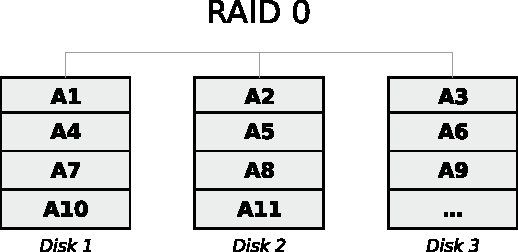
\includegraphics[]{images/raid0.pdf}

        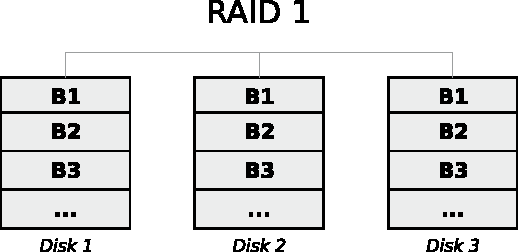
\includegraphics[]{images/raid1.pdf}

        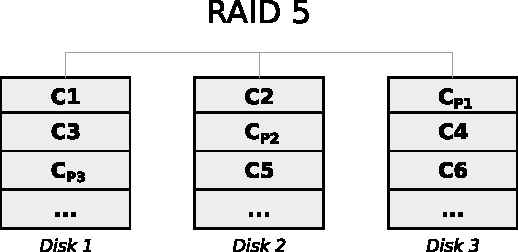
\includegraphics[]{images/raid5.pdf}
    \end{center}

    Merhere RAID-Systeme eines Typs können auch zu einem RAID-System zusammengefasst werden (z.B. \emph{RAID 100}, \emph{RAID 01}, \emph{RAID 10}, \ldots).
\end{defi}

\begin{bonus}{HDD, SSD}
    \textbf{HDD} (Hard Disk Drive, \emph{Festplatte}):
    \begin{itemize}
        \item Gehäuse der Festplatte beinhaltet mehrere, auf einer Achse übereinander montierten, runden Platten, welche mit einer magnetisierbaren Schicht überzogen sind
        \item Schreib-/Leseköpfe werden durch einen zentralen Kamm über die Platten bewegt
        \item \glqq Landing Zone\grqq zum Parken der Köpfe (Berührung $\to$ Datenverlust)
        \item Platten rotieren mit konstanter Umdrehungszahl (5400-15000 rpm)
        \item Kenngrößen:
              \subitem - kontinuierliche Übertragungsrate (\emph{sustained data rate})
              \subitem - mittlere Zugriffszeit (\emph{(data) access time}), bestehend aus:
              \subsubitem - Spurwechselzeit (\emph{seek time})
              \subsubitem - Latenzzeit (\emph{latency})
              \subsubitem - Kommando-Latenz (\emph{controller overhead})
    \end{itemize}


    \textbf{SSD} (Solid State Drive):
    \begin{itemize}
        \item keine mechanischen Bauteile
        \item niedriger Energieverbrauch
        \item hoher Datendurchsatz
        \item hoher Preis pro Speichereinheit
    \end{itemize}
\end{bonus}

\begin{bonus}{Daten- und Adressbus}
    Einzelne Komponenten sind über Leitungen, sogenannte \emph{Busse} verbunden.
    \begin{itemize}
        \item \emph{Datenbus} (bi-direktional)
        \item \emph{Adressbus} (uni-direktional, leitet Adressanfragen der CPU an RAM oder Cache weiter)
    \end{itemize}
\end{bonus}

\subsection{Parallele Rechnerarchitekturen}

\begin{defi}{Flynn'sche Klassifikation (Flynn'sche Taxonomie)}
    \begin{center}
        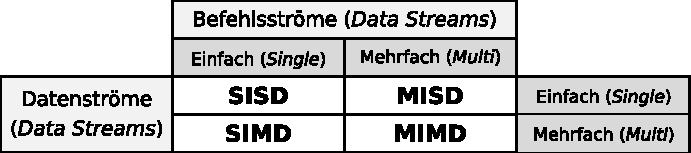
\includegraphics[]{images/flynn.pdf}
    \end{center}

    \begin{itemize}
        \item \emph{SISD} entspricht der Von-Neumann-Architektur
        \item \emph{MIMD} entspricht dem heutigen Mehrprozessorsystem
        \item \emph{SIMD} entspricht dem Aufbau einer Grafikkarte (genutzt in HPC)
        \item \emph{MISD} eher ungebräuchlich.
    \end{itemize}
\end{defi}

\begin{defi}{Shared-Memory Systeme}
    Ein \emph{Shared-Memory System} teilt den vorhandenen RAM unter den verfügbaren Prozessorenkernen auf.
    Das bedeutet, dass Daten zwischen den einzelnen Prozessorkernen \emph{implizit über den RAM} verteilt werden können, da
    jeder Kern Zugriff auf den RAM hat.

    \textbf{SMP} (\emph{symmetric multi processing}) skaliert vergleichweise schlecht.
    Das liegt daran, dass an die vorhandene Basis der Von-Neumann-Architektur einfach
    weitere Prozessorkerne angeschlossen werden. Da sich diese Prozessorkerne
    nun aber das vorhandene Bus-System teilen müssen, entsteht an dieser Stelle ein
    \emph{Flaschenhals}.

    \textbf{ccNUMA} (\emph{cache-coherent non-uniform memory architecture}) soll dieses Problem, speziell im Bereich HPC, beheben.
    Dabei wird der vorhandene Hauptspeicher auf mehrere Memory-Controller aufgeteilt.
    Jeder Prozessor ist dann an einen eigenen Memory-Controller angeschlossen.
    Dabei kann grundsätzlich weiterhin jeder Kern auf den gesamten RAM zugreifen.
    Es kann nur sein, dass der Zugriff länger dauert, wenn der betreffende Teil des RAMs von einem anderen Memory-Controller verwaltet wird.
\end{defi}

\begin{defi}{Distributed-Memory System}
    Ein \emph{Distributed-Memory System} verbindet mehrere
    \emph{unabhängige Recheneinheiten}, sodass Daten \emph{explizit} über eine Netzwerkverbindung
    zwischen dieses Recheneinheiten verteilt werden müssen.

    Dieser Ansatz skaliert sehr gut, d.h. es ist
    ohne Weiteres möglich weitere Recheneinheiten anzuschließen, ohne die Gesamtperformance
    des Systems zu beeinträchtigen
\end{defi}

\begin{bonus}{Speedup und Effizienz}
    \emph{Speed Up} und \emph{Effizienz} beurteilen die Güte paralleler Programmausführung, indem sie \emph{Zeitersparnis} und die \emph{Anzahl der verwendeten Prozessorkerne} in Relation setzen.

    Sei $T(p)$ die Zeit zur Programmausführung bei Verwendung von $p$ CPUs. Dann sind der \emph{Speed Up} $S(p)$ und die Effizienz $E(p)$ definiert wie folgt:
    $$
        S(p) = \frac{T(1)}{T(p)} \qquad  \qquad E(p) = \frac{S(p)}{p}
    $$
    Der \emph{Speed Up} gibt an, wieviel schneller die Programmausführung ist.
    Die Effizienz gibt an, wie gut die verwendeten Prozessorkerne genutzt worden sind.

    Im Idealfall ist $S(p) = p$ und $E(p) = 1$.
\end{bonus}

\begin{bonus}{Amdahl's Law}
    Nach Amdahl wird der Geschwindigkeitszuwachs vor allem durch den sequentiellen Anteil des Problems beschränkt, da sich dessen Ausführungszeit durch Parallelisierung nicht verringern lässt.

    Der \emph{Speed Up} nach Amdahl ist wie folgt definiert ($f \in (0, 1]$: serieller Teil des Programms):
    $$
        S(p) = \frac{T(1)}{f \cdot T(1) + (1-f) \cdot \frac{T(1)}{p}} = \frac{1}{f + \frac{1-f}{p}}
    $$
\end{bonus}
